\chapter{As Regras}\label{chap:regras}

\begin{itemize}
    \item[\textbf{Regra 1}] O tabuleiro começa vazio.
    \item[\textbf{Regra 2}] Preto sempre começa, e, a partir daí, Branco e Preto se alternam. 
    \item[\textbf{Regra 3}] Uma jogada consiste de colocar uma pedra de sua própria cor em uma intersecção vazia do tabuleiro, contanto que tal jogada seja legal, isto é, não conflite com as outras regras.

    \begin{figure}[h]
        \centering
        \begin{subfigure}{.3\textwidth}
            \centering
            
\includegraphics[width=.9\textwidth]{2 - Dia 1}
            \caption*{\emph{Dia.\@~1}}
        \end{subfigure}
        \begin{subfigure}{.3\textwidth}
            \centering
            
\includegraphics[width=.9\textwidth]{2 - Dia 2}
            \caption*{\emph{Dia.\@~2}}
        \end{subfigure}
        \begin{subfigure}{.3\textwidth}
            \centering
            
\includegraphics[width=.9\textwidth]{2 - Dia 3}
            \caption*{\emph{Dia.\@~3}}
        \end{subfigure}
    \end{figure}

    Os \emph{Diagramas 1 a 3} demonstram uma abertura típica no tabuleiro 9\(\times\)9. Uma vez jogadas, as pedras permanecem onde estão --- a não ser que capturadas, vide a \emph{Regra 5} ---; elas não podem ser fisicamente movidas para outros pontos. Exceto com pouquíssimas exceções causadas pela \emph{Regra 6}, uma jogada é irrestrita, isto é, você pode jogá-la onde quiser.
    \item[\textbf{Regra 4}] Um jogador pode passar o seu turno a qualquer momento.
    
    Passar geralmente ocorre em somente duas situações:
        
    \begin{enumerate}
        \item Perto do fim da partida;
        \item No início de um partida com pedras de compensação (\emph{handicap}).
    \end{enumerate}
    \item[\textbf{Regra 5}] Uma pedra ou um grupo de uma só cor conectado solidamente é capturado e removido do tabuleiro e mantido como prisioneiro quando todas as suas intersecções diretamente adjacentes são ocupadas pelo inimigo. Os 3 diagramas seguintes demonstram como capturas são executadas.
    \item[\textbf{Regra 6}] Um jogador não pode capturar suas próprias pedras. Ou seja, suicídio é ilegal.
\end{itemize}

\emph{Dia.\@~4.} Branco ocupa 3 de 4 pontos diretamente adjacentes à pedra preta; isto é, 3 de 4 liberdades. Diz-se que a pedra preta está em atari.

\emph{Dia.\@~5.} Branco 1 captura a pedra preta através da ocupação de sua última liberdade e a remove do tabuleiro.

\begin{figure}[h]
    \centering
    \begin{subfigure}{.3\textwidth}
        \centering
        
\includegraphics[width=.9\textwidth]{2 - Dia 4}
        \caption*{\emph{Dia.\@~4. Atari}}
    \end{subfigure}
    \begin{subfigure}{.3\textwidth}
        \centering
        
\includegraphics[width=.9\textwidth]{2 - Dia 5}
        \caption*{\emph{Dia.\@~5. Captura}}
    \end{subfigure}
    \begin{subfigure}{.3\textwidth}
        \centering
        
\includegraphics[width=.9\textwidth]{2 - Dia 6}
        \caption*{\emph{Dia.\@~6. Resultado}}
    \end{subfigure}
\end{figure}

\emph{Dia.\@~6.} Este é o resultado. As pedras capturadas são mantidas separadamente, tipicamente na tampa dos potes, que fica virada do avesso durante a partida.

\emph{Dia.\@~7 a 9} ilustram a captura na borda do tabuleiro.

\begin{figure}[h]
    \centering
    \begin{subfigure}{.3\textwidth}
        \centering
        
\includegraphics[width=.9\textwidth]{2 - Dia 7}
        \caption*{\emph{Dia.\@~7. Atari}}
    \end{subfigure}
    \begin{subfigure}{.3\textwidth}
        \centering
        
\includegraphics[width=.9\textwidth]{2 - Dia 8}
        \caption*{\emph{Dia.\@~8. Captura}}
    \end{subfigure}
    \begin{subfigure}{.3\textwidth}
        \centering
        
\includegraphics[width=.9\textwidth]{2 - Dia 9}
        \caption*{\emph{Dia.\@~9. Resultado}}
    \end{subfigure}
\end{figure}

\pagebreak

\emph{Dia.\@~10 a 12} ilustram a captura  no canto do tabuleiro.

\begin{figure}[h]
    \centering
    \begin{subfigure}{.3\textwidth}
        \centering
        
\includegraphics[width=.9\textwidth]{2 - Dia 10}
        \caption*{\emph{Dia.\@~10. Atari}}
    \end{subfigure}
    \begin{subfigure}{.3\textwidth}
        \centering
        
\includegraphics[width=.9\textwidth]{2 - Dia 11}
        \caption*{\emph{Dia.\@~11. Captura}}
    \end{subfigure}
    \begin{subfigure}{.3\textwidth}
        \centering
        
\includegraphics[width=.9\textwidth]{2 - Dia 12}
        \caption*{\emph{Dia.\@~12. Resultado}}
    \end{subfigure}
\end{figure}

\emph{Dia.\@~13 a 15} demonstram  como um grupo de duas pedras solidamente conectado é capturado.

\begin{figure}[h]
    \centering
    \begin{subfigure}{.3\textwidth}
        \centering
        
\includegraphics[width=.9\textwidth]{2 - Dia 13}
        \caption*{\emph{Dia.\@~13. Atari}}
    \end{subfigure}
    \begin{subfigure}{.3\textwidth}
        \centering
        
\includegraphics[width=.9\textwidth]{2 - Dia 14}
        \caption*{\emph{Dia.\@~14. Captura}}
    \end{subfigure}
    \begin{subfigure}{.3\textwidth}
        \centering
        
\includegraphics[width=.9\textwidth]{2 - Dia 15}
        \caption*{\emph{Dia.\@~15. Resultado}}
    \end{subfigure}
\end{figure}

Um grupo solidamente conectado de 5 pedras é capturado nos \emph{Dia.\@~16 a 18}.

\begin{figure}[h!]
    \centering
    \begin{subfigure}{.3\textwidth}
        \centering
        
\includegraphics[width=.9\textwidth]{2 - Dia 16}
        \caption*{\emph{Dia.\@~16. Atari}}
    \end{subfigure}
    \begin{subfigure}{.3\textwidth}
        \centering
        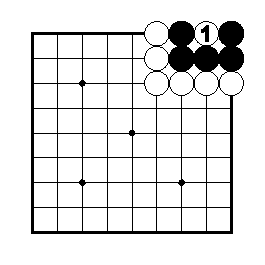
\includegraphics[width=.9\textwidth]{2 - Dia 17}
        \caption*{\emph{Dia.\@~17. Captura}}
    \end{subfigure}
    \begin{subfigure}{.3\textwidth}
        \centering
        
\includegraphics[width=.9\textwidth]{2 - Dia 18}
        \caption*{\emph{Dia.\@~18. Resultado}}
    \end{subfigure}
\end{figure}

\pagebreak

De acordo com a \emph{Regra 6}, é ilegal capturar suas próprias pedras. No \emph{Dia.\@~19}, as pedras brancas estão em atari. Não é possível salvá-las através da conexão em 1 no \emph{Dia.\@~20} pois se joga em sua própria liberdade, e as 3 pedras são deixadas sem nenhuma liberdade. Uma jogada assim é ilegal. Em outras palavras, ``a auto-captura é ilegal" ou ``o suicídio é ilegal". Entretanto, se for o turno preto, ele pode capturar as duas pedras brancas jogando em 1 no \emph{Dia.\@~21}.

\begin{figure}[h]
    \centering
    \begin{subfigure}[t]{.3\textwidth}
        \centering
        
\includegraphics[width=.9\textwidth]{2 - Dia 19}
        \caption*{\emph{Dia.\@~19. Atari}}
    \end{subfigure}
    \begin{subfigure}[t]{.3\textwidth}
        \centering
        
\includegraphics[width=.9\textwidth]{2 - Dia 20}
        \caption*{\emph{Dia.\@~20. Branco 1: ilegal}}
    \end{subfigure}
    \begin{subfigure}[t]{.3\textwidth}
        \centering
        
\includegraphics[width=.9\textwidth]{2 - Dia 21}
        \caption*{\emph{Dia.\@~21. Preto 1: legal}}
    \end{subfigure}
\end{figure}

A captura das pedras adversárias toma precedência sobre a auto-captura. No \emph{Dia 22}, as duas pedras pretas estão sob atari. Quando Branco 1 é jogado em \emph{Dia 23}, nem não há liberdades para tanto para 1 quanto para as duas pedras pretas à direita, mas são as pedras pretas, não as brancas, que são capturadas. O resultado é mostrado no \emph{Dia 24}. Se Preto quiser capturar, imediatamente, em \textbf{A}, ele pode mas não é obrigatório.

\begin{figure}[h]
    \centering
    \begin{subfigure}[t]{.3\textwidth}
        \centering
        
\includegraphics[width=.9\textwidth]{2 - Dia 22}
        \caption*{\emph{Dia.\@~22. Atari}}
    \end{subfigure}
    \begin{subfigure}[t]{.3\textwidth}
        \centering
        
\includegraphics[width=.9\textwidth]{2 - Dia 23}
        \caption*{\emph{Dia.\@~23. Branco captura}}
    \end{subfigure}
    \begin{subfigure}[t]{.3\textwidth}
        \centering
        
\includegraphics[width=.9\textwidth]{2 - Dia 24}
        \caption*{\emph{Dia.\@~24. Resultado}}
    \end{subfigure}
\end{figure}

\pagebreak

\section{30 Problemas de Captura e Resgate de Pedras}

Aqui estão 30 problemas. Depois de pensar sobre eles, você entenderá completamente tanto como capturar pedras quanto, também, resgatar pedras em risco.

\begin{figure}[h!]
    \centering
    \captionsetup{justification=raggedright,singlelinecheck=false}
    \begin{subfigure}[t]{.3\textwidth}
        
\includegraphics[width=.9\textwidth]{2 - Problema 1}
        \caption*{\textbf{Problema 1}: \emph{Preto a capturar uma pedra}}
    \end{subfigure}
    \hfill
    \begin{subfigure}[t]{.3\textwidth}
        
\includegraphics[width=.9\textwidth]{2 - Problema 2}
        \caption*{\textbf{Problema 2}: \emph{Preto a capturar uma pedra}}
    \end{subfigure}
    \hfill
    \begin{subfigure}[t]{.3\textwidth}
        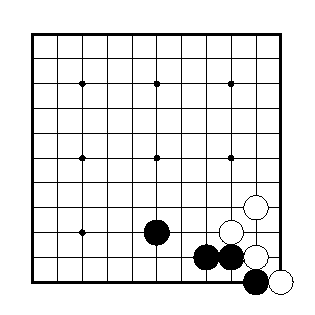
\includegraphics[width=.9\textwidth]{2 - Problema 3}
        \caption*{\textbf{Problema 3}: \emph{Preto a capturar uma pedra}}
    \end{subfigure}
    \par\bigskip
    \begin{subfigure}[t]{.3\textwidth}
        
\includegraphics[width=.9\textwidth]{2 - Problema 4}
        \caption*{\textbf{Problema 4}: \emph{Preto a capturar duas pedras}}
    \end{subfigure}
    \hfill
    \begin{subfigure}[t]{.3\textwidth}
        
\includegraphics[width=.9\textwidth]{2 - Problema 5}
        \caption*{\textbf{Problema 5}: \emph{Preto a capturar duas pedras}}
    \end{subfigure}
    \hfill
    \begin{subfigure}[t]{.3\textwidth}
        
\includegraphics[width=.9\textwidth]{2 - Problema 6}
        \caption*{\textbf{Problema 6}: \emph{Preto a capturar duas pedras}}
    \end{subfigure}
    \par\bigskip
    \begin{subfigure}[t]{.3\textwidth}
        
\includegraphics[width=.9\textwidth]{2 - Problema 7}
        \caption*{\textbf{Problema 7}: \emph{Preto a capturar duas pedras}}
    \end{subfigure}
    \hfill
    \begin{subfigure}[t]{.3\textwidth}
        
\includegraphics[width=.9\textwidth]{2 - Problema 8}
        \caption*{\textbf{Problema 8}: \emph{Preto a capturar duas pedras}}
    \end{subfigure}
    \hfill
    \begin{subfigure}[t]{.3\textwidth}
        
\includegraphics[width=.9\textwidth]{2 - Problema 9}
        \caption*{\textbf{Problema 9}: \emph{Preto a capturar três pedras}}
    \end{subfigure}
\end{figure}

\begin{figure}[p!]
    \centering
    \captionsetup{justification=raggedright,singlelinecheck=false}
    \begin{subfigure}[t]{.3\textwidth}
        
\includegraphics[width=.9\textwidth]{2 - Problema 10}
        \caption*{\textbf{Problema 10}: \emph{Preto a capturar três pedra}}
    \end{subfigure}
    \hfill
    \begin{subfigure}[t]{.3\textwidth}
        
\includegraphics[width=.9\textwidth]{2 - Problema 11}
        \caption*{\textbf{Problema 11}: \emph{Preto a capturar três pedra}}
    \end{subfigure}
    \hfill
    \begin{subfigure}[t]{.3\textwidth}
        
\includegraphics[width=.9\textwidth]{2 - Problema 12}
        \caption*{\textbf{Problema 12}: \emph{Preto a capturar uma pedra}}
    \end{subfigure}
    \par\bigskip
    \begin{subfigure}[t]{.3\textwidth}
        
\includegraphics[width=.9\textwidth]{2 - Problema 13}
        \caption*{\textbf{Problema 13}: \emph{Preto a capturar cinco pedras}}
    \end{subfigure}
    \hfill
    \begin{subfigure}[t]{.3\textwidth}
        
\includegraphics[width=.9\textwidth]{2 - Problema 14}
        \caption*{\textbf{Problema 14}: \emph{Preto a capturar cinco pedras}}
    \end{subfigure}
    \hfill
    \begin{subfigure}[t]{.3\textwidth}
        
\includegraphics[width=.9\textwidth]{2 - Problema 15}
        \caption*{\textbf{Problema 15}: \emph{Resgate a pedra marcada}}
    \end{subfigure}
    \par\bigskip
    \begin{subfigure}[t]{.3\textwidth}
        
\includegraphics[width=.9\textwidth]{2 - Problema 16}
        \caption*{\textbf{Problema 16}: \emph{Resgate a pedra marcada}}
    \end{subfigure}
    \hfill
    \begin{subfigure}[t]{.3\textwidth}
        
\includegraphics[width=.9\textwidth]{2 - Problema 17}
        \caption*{\textbf{Problema 17}: \emph{Resgate as pedras marcadas}}
    \end{subfigure}
    \hfill
    \begin{subfigure}[t]{.3\textwidth}
        
\includegraphics[width=.9\textwidth]{2 - Problema 18}
        \caption*{\textbf{Problema 18}: \emph{Resgate a pedra marcada}}
    \end{subfigure}
    \par\bigskip
    \begin{subfigure}[t]{.3\textwidth}
        
\includegraphics[width=.9\textwidth]{2 - Problema 19}
        \caption*{\textbf{Problema 19}: \emph{Resgate as pedras marcadas}}
    \end{subfigure}
    \hfill
    \begin{subfigure}[t]{.3\textwidth}
        
\includegraphics[width=.9\textwidth]{2 - Problema 20}
        \caption*{\textbf{Problema 20}: \emph{Resgate as pedras marcadas}}
    \end{subfigure}
    \hfill
    \begin{subfigure}[t]{.3\textwidth}
        
\includegraphics[width=.9\textwidth]{2 - Problema 21}
        \caption*{\textbf{Problema 21}: \emph{Resgate as pedras marcadas}}
    \end{subfigure}
\end{figure}

\begin{figure}[p!]
    \centering
    \captionsetup{justification=raggedright,singlelinecheck=false}
    \begin{subfigure}[t]{.3\textwidth}
        
\includegraphics[width=.9\textwidth]{2 - Problema 22}
        \caption*{\textbf{Problema 22}: \emph{Será que Branco consegue resgatar as pedras marcadas?}}
    \end{subfigure}
    \hfill
    \begin{subfigure}[t]{.3\textwidth}
        
\includegraphics[width=.9\textwidth]{2 - Problema 23}
        \caption*{\textbf{Problema 23}: \emph{Como Preto deveria fazer atari às pedras marcadas?}}
    \end{subfigure}
    \hfill
    \begin{subfigure}[t]{.3\textwidth}
        
\includegraphics[width=.9\textwidth]{2 - Problema 24}
        \caption*{\textbf{Problema 24}: \emph{Como Preto deveria fazer atari às pedras marcadas?}}
    \end{subfigure}
    \par\bigskip
    \begin{subfigure}[t]{.3\textwidth}
        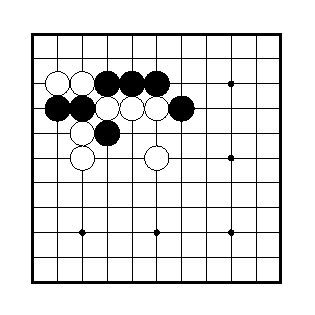
\includegraphics[width=.9\textwidth]{2 - Problema 25}
        \caption*{\textbf{Problema 25}: \emph{Preto a capturar três pedras}}
    \end{subfigure}
    \hfill
    \begin{subfigure}[t]{.3\textwidth}
        
\includegraphics[width=.9\textwidth]{2 - Problema 26}
        \caption*{\textbf{Problema 26}: \emph{Preto a capturar quatro pedras}}
    \end{subfigure}
    \hfill
    \begin{subfigure}[t]{.3\textwidth}
        \includegraphics[width=.9\textwidth]{2 - Problema 27}
        \caption*{\textbf{Problema 27}: \emph{Preto a capturar três pedras}}
    \end{subfigure}
    \par\bigskip
    \begin{subfigure}[t]{.3\textwidth}
        \includegraphics[width=.9\textwidth]{2 - Problema 28}
        \caption*{\textbf{Problema 28}: \emph{Onde Preto deveria jogar?}}
    \end{subfigure}
    \hfill
    \begin{subfigure}[t]{.3\textwidth}
        \includegraphics[width=.9\textwidth]{2 - Problema 29}
        \caption*{\textbf{Problema 29}: \emph{Como Preto pode capturar uma pedra?}}
    \end{subfigure}
    \hfill
    \begin{subfigure}[t]{.3\textwidth}
        \includegraphics[width=.9\textwidth]{2 - Problema 30}
        \caption*{\textbf{Problema 30}: \emph{Como Preto pode capturar uma pedra?}}
    \end{subfigure}
\end{figure}

\pagebreak

\section{Respostas aos Problemas de 1 a 30}

\begin{SCfigure}[][h!]
    \begin{subfigure}[t]{.31\textwidth}
        \includegraphics[width=1\textwidth]{2 - Problema 1 - Dia 1}
        \caption*{\emph{Dia.\@~1. Correto}}
    \end{subfigure}
    \hfill
    \begin{subfigure}[t]{.31\textwidth}
        \includegraphics[width=1\textwidth]{2 - Problema 1 - Dia 2}
        \caption*{\emph{Dia.\@~2. Errado}}
    \end{subfigure}
    \hfill
    \caption*{\textbf{Resposta ao Problema 1}\\\\Preto 1 no \emph{Dia.\@~1} captura um pedra.\\\\Se Preto joga 1 no \emph{Dia.\@~2}, Branco pode resgatar sua pedra através da extensão de 2.}
\end{SCfigure}

\vfill

\begin{SCfigure}[][h!]
    \begin{subfigure}[t]{.31\textwidth}
        \includegraphics[width=1\textwidth]{2 - Problema 2 - Dia 1}
        \caption*{\emph{Dia.\@~1. Correto}}
    \end{subfigure}
    \hfill
    \begin{subfigure}[t]{.31\textwidth}
        \includegraphics[width=1\textwidth]{2 - Problema 2 - Dia 2}
        \caption*{\emph{Dia.\@~2. Errado}}
    \end{subfigure}
    \hfill
    \caption*{\textbf{Resposta ao Problema 2}\\\\Preto 1 no \emph{Dia.\@~1} captura uma pedra.\\\\Se Preto conecta em 1 no \emph{Dia.\@~2}, Branco pode resgatar sua pedra conectando em 2.}
\end{SCfigure}

\vfill

\begin{SCfigure}[][h!]
    \begin{subfigure}[t]{.31\textwidth}
        \includegraphics[width=1\textwidth]{2 - Problema 3 - Dia 1}
        \caption*{\emph{Dia.\@~1. Correto}}
    \end{subfigure}
    \hfill
    \begin{subfigure}[t]{.31\textwidth}
        \includegraphics[width=1\textwidth]{2 - Problema 3 - Dia 2}
        \caption*{\emph{Dia.\@~2. Errado}}
    \end{subfigure}
    \hfill
    \caption*{\textbf{Resposta ao Problema 3}\\\\Preto 1 no \emph{Dia.\@~1} captura uma pedra.\\\\Se Preto conecta em 1 no \emph{Dia.\@~2}, Branco pode resgatar sua pedra conectando em 2.}
\end{SCfigure}

\pagebreak

\begin{SCfigure}[][h!]
    \begin{subfigure}[t]{.31\textwidth}
        \includegraphics[width=1\textwidth]{2 - Problema 4 - Dia 1}
        \caption*{\emph{Dia.\@~1. Correto}}
    \end{subfigure}
    \hfill
    \begin{subfigure}[t]{.31\textwidth}
        \includegraphics[width=1\textwidth]{2 - Problema 4 - Dia 2}
        \caption*{\emph{Dia.\@~2. Errado}}
    \end{subfigure}
    \hfill
    \caption*{\textbf{Resposta ao Problema 4}\\\\Preto 1 no \emph{Dia.\@~1} captura duas pedras.\\\\Se Preto joga 1 no \emph{Dia.\@~2}, Branco pode resgatar suas pedras estendendo em 2.}
\end{SCfigure}

\vfill

\begin{SCfigure}[][h!]
    \begin{subfigure}[t]{.31\textwidth}
        \includegraphics[width=1\textwidth]{2 - Problema 5 - Dia 1}
        \caption*{\emph{Dia.\@~1. Correto}}
    \end{subfigure}
    \hfill
    \begin{subfigure}[t]{.31\textwidth}
        \includegraphics[width=1\textwidth]{2 - Problema 5 - Dia 2}
        \caption*{\emph{Dia.\@~2. Errado}}
    \end{subfigure}
    \hfill
    \caption*{\textbf{Resposta ao Problema 5}\\\\Preto 1 no \emph{Dia.\@~1} captura duas pedras.\\\\Se Preto estende para 1 no \emph{Dia.\@~2}, Branco pode resgatar suas pedras conectando em 2.}
\end{SCfigure}

\vfill

\begin{SCfigure}[][h!]
    \begin{subfigure}[t]{.31\textwidth}
        \includegraphics[width=1\textwidth]{2 - Problema 6 - Dia 1}
        \caption*{\emph{Dia.\@~1. Correto}}
    \end{subfigure}
    \hfill
    \begin{subfigure}[t]{.31\textwidth}
        \includegraphics[width=1\textwidth]{2 - Problema 6 - Dia 2}
        \caption*{\emph{Dia.\@~2. Errado}}
    \end{subfigure}
    \hfill
    \caption*{\textbf{Resposta ao Problema 6}\\\\Preto 1 no \emph{Dia.\@~1} captura as duas pedras marcadas.\\\\Se Preto estende para 1 no \emph{Dia.\@~2}, Branco pode resgatar suas duas pedras capturando as duas pedras pretas com 2.}
\end{SCfigure}

\pagebreak

\begin{SCfigure}[][h!]
    \begin{subfigure}[t]{.31\textwidth}
        \includegraphics[width=1\textwidth]{2 - Problema 7 - Dia 1}
        \caption*{\emph{Dia.\@~1. Correto}}
    \end{subfigure}
    \hfill
    \begin{subfigure}[t]{.31\textwidth}
        \includegraphics[width=1\textwidth]{2 - Problema 7 - Dia 2}
        \caption*{\emph{Dia.\@~2. Errado}}
    \end{subfigure}
    \hfill
    \caption*{\textbf{Resposta ao Problema 7}\\\\Preto 1 no \emph{Dia.\@~1} captura duas pedras.\\\\Se Preto faz atari com 1 em \emph{Dia.\@~2}, Branco pode resgatar suas pedras e capturar duas do Preto com 2.}
\end{SCfigure}

\vfill

\begin{SCfigure}[][h!]
    \begin{subfigure}[t]{.31\textwidth}
        \includegraphics[width=1\textwidth]{2 - Problema 8 - Dia 1}
        \caption*{\emph{Dia.\@~1. Correto}}
    \end{subfigure}
    \hfill
    \begin{subfigure}[t]{.31\textwidth}
        \includegraphics[width=1\textwidth]{2 - Problema 8 - Dia 2}
        \caption*{\emph{Dia.\@~2. Errado}}
    \end{subfigure}
    \hfill
    \caption*{\textbf{Resposta ao Problema 8}\\\\Preto 1 no \emph{Dia.\@~1} captura duas pedras.\\\\\emph{Dia.\@~2} mostra o resultado desta captura.}
\end{SCfigure}

\vfill

\begin{SCfigure}[][h!]
    \begin{subfigure}[t]{.31\textwidth}
        \includegraphics[width=1\textwidth]{2 - Problema 9 - Dia 1}
        \caption*{\emph{Dia.\@~1. Correto}}
    \end{subfigure}
    \hfill
    \begin{subfigure}[t]{.31\textwidth}
        \includegraphics[width=1\textwidth]{2 - Problema 9 - Dia 2}
        \caption*{\emph{Dia.\@~2. Errado}}
    \end{subfigure}
    \hfill
    \caption*{\textbf{Resposta ao Problema 9}\\\\Preto 1 no \emph{Dia.\@~1} captura três pedras.\\\\
    Se Preto conecta em 1 no \emph{Dia.\@~2}, Branco pode resgatar sua pedra conectando em 2.}
\end{SCfigure}

\pagebreak

\begin{SCfigure}[][h!]
    \begin{subfigure}[t]{.31\textwidth}
        \includegraphics[width=1\textwidth]{2 - Problema 10 - Dia 1}
        \caption*{\emph{Dia.\@~1. Correto}}
    \end{subfigure}
    \hfill
    \begin{subfigure}[t]{.31\textwidth}
        \includegraphics[width=1\textwidth]{2 - Problema 10 - Dia 2}
        \caption*{\emph{Dia.\@~2. Errado}}
    \end{subfigure}
    \hfill
    \caption*{\textbf{Resposta ao Problema 10}\\\\Preto 1 no \emph{Dia.\@~1} captura três pedras.\\\\Se Preto joga 1 no \emph{Dia.\@~2}, Branco pode resgatar as pedras em risco com a conexão em 2.}
\end{SCfigure}

\vfill

\begin{SCfigure}[][h!]
    \begin{subfigure}[t]{.31\textwidth}
        \includegraphics[width=1\textwidth]{2 - Problema 11 - Dia 1}
        \caption*{\emph{Dia.\@~1. Correto}}
    \end{subfigure}
    \hfill
    \begin{subfigure}[t]{.31\textwidth}
        \includegraphics[width=1\textwidth]{2 - Problema 11 - Dia 2}
        \caption*{\emph{Dia.\@~2. Errado}}
    \end{subfigure}
    \hfill
    \caption*{\textbf{Resposta ao Problema 11}\\\\Preto 1 no \emph{Dia.\@~1} captura três pedras.\\\\Se Preto joga 1 no \emph{Dia.\@~2}, Branco pode salvar suas pedras e capturar as 4 pretas com 2.}
\end{SCfigure}

\vfill

\begin{SCfigure}[][h!]
    \begin{subfigure}[t]{.31\textwidth}
        \includegraphics[width=1\textwidth]{2 - Problema 12 - Dia 1}
        \caption*{\emph{Dia.\@~1. Correto}}
    \end{subfigure}
    \hfill
    \begin{subfigure}[t]{.31\textwidth}
        \includegraphics[width=1\textwidth]{2 - Problema 12 - Dia 2}
        \caption*{\emph{Dia.\@~2. Errado}}
    \end{subfigure}
    \hfill
    \caption*{\textbf{Resposta ao Problema 12}\\\\Preto 1 em \emph{Dia.\@~1} captura uma pedra (crucial).\\\\Se Preto estende para 1 no \emph{Dia.\@~2}, Branco pode resgatar sua pedra conectando em 2.}
\end{SCfigure}

\pagebreak

\begin{SCfigure}[][h!]
    \begin{subfigure}[t]{.31\textwidth}
        \includegraphics[width=1\textwidth]{2 - Problema 13 - Dia 1}
        \caption*{\emph{Dia.\@~1. Correto}}
    \end{subfigure}
    \hfill
    \begin{subfigure}[t]{.31\textwidth}
        \includegraphics[width=1\textwidth]{2 - Problema 13 - Dia 2}
        \caption*{\emph{Dia.\@~2. Errado}}
    \end{subfigure}
    \hfill
    \caption*{\textbf{Resposta ao Problema 13}\\\\Preto 1 no \emph{Dia.\@~1} captura cinco pedras.\\\\Se Preto joga 1 em \emph{Dia.\@~2} para escapar do atari, Branco pode resgatar suas cinco pedras conectando em 2.}
\end{SCfigure}

\vfill

\begin{SCfigure}[][h!]
    \begin{subfigure}[t]{.31\textwidth}
        \includegraphics[width=1\textwidth]{2 - Problema 14 - Dia 1}
        \caption*{\emph{Dia.\@~1. Correto}}
    \end{subfigure}
    \hfill
    \begin{subfigure}[t]{.31\textwidth}
        \includegraphics[width=1\textwidth]{2 - Problema 14 - Dia 2}
        \caption*{\emph{Dia.\@~2. Errado}}
    \end{subfigure}
    \hfill
    \caption*{\textbf{Resposta ao Problema 14}\\\\Preto 1 no \emph{Dia.\@~1} captura cinco pedras.\\\\Se Preto conecta em 1 no \emph{Dia.\@~2}, Branco pode resgatar suas cinco pedras capturando quatro pedras com 2.}
\end{SCfigure}

\vfill

\begin{SCfigure}[][h!]
    \begin{subfigure}[t]{.31\textwidth}
        \includegraphics[width=1\textwidth]{2 - Problema 15 - Dia 1}
        \caption*{\emph{Dia.\@~1. Correto}}
    \end{subfigure}
    \hfill
    \begin{subfigure}[t]{.31\textwidth}
        \includegraphics[width=1\textwidth]{2 - Problema 15 - Dia 2}
        \caption*{\emph{Dia.\@~2. Errado}}
    \end{subfigure}
    \hfill
    \caption*{\textbf{Resposta ao Problema 15}\\\\Preto pode resgatar sua pedra sob atari conectando em 1 no \emph{Dia.\@~1}.\\\\Se Preto faz atari com 1 no \emph{Dia.\@~2}, Branco pode capturar com 2.}
\end{SCfigure}

\pagebreak

\begin{SCfigure}[][h!]
    \begin{subfigure}[t]{.31\textwidth}
        \includegraphics[width=1\textwidth]{2 - Problema 16 - Dia 1}
        \caption*{\emph{Dia.\@~1. Correto}}
    \end{subfigure}
    \hfill
    \begin{subfigure}[t]{.31\textwidth}
        \includegraphics[width=1\textwidth]{2 - Problema 16 - Dia 2}
        \caption*{\emph{Dia.\@~2. Errado}}
    \end{subfigure}
    \hfill
    \caption*{\textbf{Resposta ao Problema 16}\\\\Preto 1 no \emph{Dia.\@~1} resgata sua pedra em atari.\\\\Se Preto faz atari com 1 no \emph{Dia.\@~2}, Branco pode capturar uma pedra (crucial) com 2.}
\end{SCfigure}

\vfill

\begin{SCfigure}[][h!]
    \begin{subfigure}[t]{.31\textwidth}
        \includegraphics[width=1\textwidth]{2 - Problema 17 - Dia 1}
        \caption*{\emph{Dia.\@~1. Correto}}
    \end{subfigure}
    \hfill
    \begin{subfigure}[t]{.31\textwidth}
        \includegraphics[width=1\textwidth]{2 - Problema 17 - Dia 2}
        \caption*{\emph{Dia.\@~2. Errado}}
    \end{subfigure}
    \hfill
    \caption*{\textbf{Resposta ao Problema 17}\\\\Preto 1 no \emph{Dia.\@~1} salva suas duas pedras sob atari.\\\\Se Preto faz atari com 1 no \emph{Dia.\@~2}, Branco pode capturar duas pedras com 2.}
\end{SCfigure}

\vfill

\begin{SCfigure}[][h!]
    \begin{subfigure}[t]{.31\textwidth}
        \includegraphics[width=1\textwidth]{2 - Problema 18 - Dia 1}
        \caption*{\emph{Dia.\@~1. Correto}}
    \end{subfigure}
    \hfill
    \begin{subfigure}[t]{.31\textwidth}
        \includegraphics[width=1\textwidth]{2 - Problema 18 - Dia 2}
        \caption*{\emph{Dia.\@~2. Errado}}
    \end{subfigure}
    \hfill
    \caption*{\textbf{Resposta ao Problema 18}\\\\Preto 1 no \emph{Dia.\@~1} resgata sua pedra em atari.\\\\Se Preto faz atari com 1 no \emph{Dia.\@~2}, Branco pode capturar uma pedra com 2.}
\end{SCfigure}

\pagebreak

\begin{SCfigure}[][h!]
    \begin{subfigure}[t]{.31\textwidth}
        \includegraphics[width=1\textwidth]{2 - Problema 19 - Dia 1}
        \caption*{\emph{Dia.\@~1. Correto}}
    \end{subfigure}
    \hfill
    \begin{subfigure}[t]{.31\textwidth}
        \includegraphics[width=1\textwidth]{2 - Problema 19 - Dia 2}
        \caption*{\emph{Dia.\@~2. Errado}}
    \end{subfigure}
    \hfill
    \caption*{\textbf{Resposta ao Problema 19}\\\\Preto 1 no \emph{Dia.\@~1} resgata suas três pedras em atari.\\\\Se Preto faz atari com 1 no \emph{Dia.\@~2}, Branco pode capturar três pedras com 2.}
\end{SCfigure}

\vfill

\begin{SCfigure}[][h!]
    \begin{subfigure}[t]{.31\textwidth}
        \includegraphics[width=1\textwidth]{2 - Problema 20 - Dia 1}
        \caption*{\emph{Dia.\@~1. Correto}}
    \end{subfigure}
    \hfill
    \begin{subfigure}[t]{.31\textwidth}
        \includegraphics[width=1\textwidth]{2 - Problema 20 - Dia 2}
        \caption*{\emph{Dia.\@~2. Errado}}
    \end{subfigure}
    \hfill
    \caption*{\textbf{Resposta ao Problema 20}\\\\Preto 1 no \emph{Dia.\@~1} resgata suas três pedras em atari.\\\\Se Preto faz atari com 1 no \emph{Dia.\@~2}, Branco pode capturar três pedras com 2.}
\end{SCfigure}

\vfill

\begin{SCfigure}[][h!]
    \begin{subfigure}[t]{.31\textwidth}
        \includegraphics[width=1\textwidth]{2 - Problema 21 - Dia 1}
        \caption*{\emph{Dia.\@~1. Correto}}
    \end{subfigure}
    \hfill
    \begin{subfigure}[t]{.31\textwidth}
        \includegraphics[width=1\textwidth]{2 - Problema 21 - Dia 2}
        \caption*{\emph{Dia.\@~2. Errado}}
    \end{subfigure}
    \hfill
    \caption*{\textbf{Resposta ao Problema 21}\\\\Preto 1 no \emph{1} resgata suas duas pedras em atari.\\\\Se Preto faz atari com 1 no \emph{Dia.\@~2}, Branco captura duas pedras com 2.}
\end{SCfigure}

\pagebreak

\begin{SCfigure}[][h!]
    \begin{subfigure}[t]{.31\textwidth}
        \includegraphics[width=1\textwidth]{2 - Problema 22 - Dia 1}
        \caption*{\emph{Dia.\@~1. Correto}}
    \end{subfigure}
    \hfill
    \begin{subfigure}[t]{.31\textwidth}
        \includegraphics[width=1\textwidth]{2 - Problema 22 - Dia 2}
        \caption*{\emph{Dia.\@~2. Errado}}
    \end{subfigure}
    \hfill
    \caption*{\textbf{Resposta ao Problema 22}\\\\Branco não consegue escapar. Se ele rastejar na primeira linha com 1 a 10 no \emph{Dia.\@~1}, Preto captura oito pedras com 12.\\\\Após Branco 1 no \emph{Dia 2}, se Preto faz atari a partir da direita com 2, Branco pode escapar com 3 e 5.}
\end{SCfigure}

\vfill

\begin{SCfigure}[][h!]
    \begin{subfigure}[t]{.31\textwidth}
        \includegraphics[width=1\textwidth]{2 - Problema 23 - Dia 1}
        \caption*{\emph{Dia.\@~1. Correto}}
    \end{subfigure}
    \hfill
    \begin{subfigure}[t]{.31\textwidth}
        \includegraphics[width=1\textwidth]{2 - Problema 23 - Dia 2}
        \caption*{\emph{Dia.\@~2. Errado}}
    \end{subfigure}
    \hfill
    \caption*{\textbf{Resposta ao Problema 23}\\\\Preto precisa fazer atari com 1 no \emph{Dia.\@~1}. Se Branco 2, Preto captura duas pedras com 3.\\\\Se Preto faz atari a partir da direita com 1 no \emph{Dia.\@~2}, ele possui somente uma liberdade, então Branco pode capturar três pedras com 2.}
\end{SCfigure}

\vfill

\begin{SCfigure}[][h!]
    \begin{subfigure}[t]{.31\textwidth}
        \includegraphics[width=1\textwidth]{2 - Problema 24 - Dia 1}
        \caption*{\emph{Dia.\@~1. Correto}}
    \end{subfigure}
    \hfill
    \begin{subfigure}[t]{.31\textwidth}
        \includegraphics[width=1\textwidth]{2 - Problema 24 - Dia 2}
        \caption*{\emph{Dia.\@~2. Errado}}
    \end{subfigure}
    \hfill
    \caption*{\textbf{Resposta ao Problema 24}\\\\Preto precisa fazer atari com 1 no \emph{Dia.\@~1}. Se Branco 2, Preto faz atari novamente e suas pedras estão seguras. Se Branco \textbf{A}, Preto captura em \textbf{B}.\\\\Se Preto faz atari pelo topo com 1 em \emph{Dia.\@~2}, após Branco 2, as pedras marcadas ficam encarceradas.}
\end{SCfigure}

\pagebreak

\begin{SCfigure}[][h!]
    \begin{subfigure}[t]{.31\textwidth}
        \includegraphics[width=1\textwidth]{2 - Problema 25 - Dia 1}
        \caption*{\emph{Dia.\@~1. Correto}}
    \end{subfigure}
    \hfill
    \begin{subfigure}[t]{.31\textwidth}
        \includegraphics[width=1\textwidth]{2 - Problema 25 - Dia 2}
        \caption*{\emph{Dia.\@~2. Errado}}
    \end{subfigure}
    \hfill
    \caption*{\textbf{Resposta ao Problema 25}\\\\Preto precisa fazer atari com 1 no \emph{Dia.\@~1}. Ele pode agora capturar três pedras com \textbf{A}. Se Branco \textbf{A}, suas pedras ainda estão sob atari.\\\\Se Preto faz atari com 1 no \emph{Dia.\@~2}, Branco conecta com 2 e suas pedras escapam.}
\end{SCfigure}

\vfill


\begin{SCfigure}[][h!]
    \begin{subfigure}[t]{.31\textwidth}
        \includegraphics[width=1\textwidth]{2 - Problema 26 - Dia 1}
        \caption*{\emph{Dia.\@~1. Correto}}
    \end{subfigure}
    \hfill
    \begin{subfigure}[t]{.31\textwidth}
        \includegraphics[width=1\textwidth]{2 - Problema 26 - Dia 2}
        \caption*{\emph{Dia.\@~2. Errado}}
    \end{subfigure}
    \hfill
    \caption*{\textbf{Resposta ao Problema 25}\\\\Se Preto faz atari em 1 no \emph{Dia.\@~1}, ele captura quatro pedras. Se Branco joga 2, ele não possuirá nenhuma maneira de escapar depois de Preto 3.\\\\Se Preto faz atari com 1 no \emph{Dia.\@~2}, Branco estende com 2 e suas pedras escapam.}
\end{SCfigure}

\vfill

\begin{SCfigure}[][h!]
    \begin{subfigure}[t]{.31\textwidth}
        \includegraphics[width=1\textwidth]{2 - Problema 27 - Dia 1}
        \caption*{\emph{Dia.\@~1. Correto}}
    \end{subfigure}
    \hfill
    \begin{subfigure}[t]{.31\textwidth}
        \includegraphics[width=1\textwidth]{2 - Problema 27 - Dia 2}
        \caption*{\emph{Dia.\@~2. Errado}}
    \end{subfigure}
    \hfill
    \caption*{\textbf{Resposta ao Problema 27}\\\\Preto deveria fazer atari com 1 no \emph{Dia.\@~1}. Preto pode agora capturar três pedras jogando em \textbf{A}. Se Branco \textbf{A}, suas pedras ainda estão em atari.\\\\Se Preto faz atari com 1 no \emph{Dia.\@~2}, Branco conecta com 2 e suas pedras escaparam.}
\end{SCfigure}

\pagebreak

\begin{SCfigure}[][h!]
    \begin{subfigure}[t]{.31\textwidth}
        \includegraphics[width=1\textwidth]{2 - Problema 28 - Dia 1}
        \caption*{\emph{Dia.\@~1. Correto}}
    \end{subfigure}
    \hfill
    \begin{subfigure}[t]{.31\textwidth}
        \includegraphics[width=1\textwidth]{2 - Problema 28 - Dia 2}
        \caption*{\emph{Dia.\@~2. Errado}}
    \end{subfigure}
    \hfill
    \caption*{\textbf{Resposta ao Problema 28}\\\\As pedras pretas à direita estão em perigo, então ele precisa fazer atari na pedra marcada com 1 no \emph{Dia.\@~1}.\\\\Se Preto faz atari vindo debaixo com 1 no \emph{Dia.\@~2}, Branco faz atari com 2 e pode capturar em seguida com \textbf{A}.}
\end{SCfigure}

\vfill

\begin{SCfigure}[][h!]
    \begin{subfigure}[t]{.31\textwidth}
        \includegraphics[width=1\textwidth]{2 - Problema 29 - Dia 1}
        \caption*{\emph{Dia.\@~1. Correto}}
    \end{subfigure}
    \hfill
    \begin{subfigure}[t]{.31\textwidth}
        \includegraphics[width=1\textwidth]{2 - Problema 29 - Dia 2}
        \caption*{\emph{Dia.\@~2. Errado}}
    \end{subfigure}
    \hfill
    \caption*{\textbf{Resposta ao Problema 30}\\\\Preto precisa fazer um duplo-atari  nas pedras marcadas com 1 no \emph{Dia.\@~1}. Ele pode agora capturar uma pedra em \textbf{A} ou \textbf{B}.\\\\Preto 1 em \emph{Dia 2} faz atari em somente uma pedra branca. Branco conecta com 2 e Preto não pode capturar nada.}
\end{SCfigure}

\vfill

\begin{SCfigure}[][h!]
    \begin{subfigure}[t]{.31\textwidth}
        \includegraphics[width=1\textwidth]{2 - Problema 29 - Dia 1}
        \caption*{\emph{Dia.\@~1. Correto}}
    \end{subfigure}
    \hfill
    \begin{subfigure}[t]{.31\textwidth}
        \includegraphics[width=1\textwidth]{2 - Problema 29 - Dia 2}
        \caption*{\emph{Dia.\@~2. Errado}}
    \end{subfigure}
    \hfill
    \caption*{\textbf{Resposta ao Problema 30}\\\\Preto 1 no \emph{Dia.\@~1} é um duplo-atari, então Branco pode capturar uma das pedras marcadas em \textbf{A} ou \textbf{B}.\\\\Preto 1 no \emph{Dia.\@~2} faz atari em somente uma pedra. Branco conecta com 2 e Preto não pode capturar nada.}
\end{SCfigure}